\documentclass[12pt]{report}

\usepackage[T1]{fontenc}
\usepackage[utf8]{inputenc}

% Math
\usepackage{amsmath}
\usepackage{amsfonts}
\usepackage{amssymb}
\usepackage{amsthm}

% Algorithm & code listing
\usepackage{algorithm}
\usepackage[noend]{algpseudocode}
\makeatletter
\algrenewcommand\ALG@beginalgorithmic{\footnotesize}
\def\NoNumber#1{{\def\alglinenumber##1{}\State #1}\addtocounter{ALG@line}{-1}}
\usepackage{titling}
\usepackage{listings}
\usepackage{enumitem}

% Graphics & figures
\usepackage{graphicx}
\usepackage[pdf]{graphviz}
\usepackage{tikz}
\usetikzlibrary{automata,arrows,positioning,calc}
\usepackage{forest}
\usepackage{geometry}
\usepackage{changepage}
% Utils
\usepackage{caption}
\usepackage{subcaption}
\usepackage[hidelinks]{hyperref}
\usepackage{courier}
\usepackage{subfloat}
\usepackage{enumitem}

% Bibliotheq
\usepackage{biblatex}
\addbibresource{thesis.bib}

\lstset{basicstyle=\ttfamily\footnotesize,breaklines=true}

% MACROS
\newcommand*{\QED}{\hfill\ensuremath{\square}}
\newcommand{\stirlingii}{\genfrac{\{}{\}}{0pt}{}}

\newtheoremstyle{break}
{\topsep}{\topsep}%
{\itshape}{}%
{\bfseries}{}%
{\newline}{}%
\theoremstyle{break}
\newtheorem{definition}{Definition}[section]
\newtheorem{theorem}{Theorem}
\newtheorem{lemma}[theorem]{Lemma}
\newtheorem{example}[theorem]{Example}
\newtheorem{corollary}{Corollary}[theorem]

\newcommand{\subtitle}[1]{%
  \posttitle{%
    \par\end{center}
  \begin{center}\large#1\end{center}
  \vskip0.5em}%
}

\begin{document}

%%%%%%%%%%%%%%%%%%%%%%%% Title Page %%%%%%%%%%%%%%%%%%%%%%%%
\begin{titlepage}
  \begin{center}
    {\LARGE \textbf{Bayesian Parameter Inference of Markov Population Model.}}
    \\[1cm]
    {\Large \textbf{Master Thesis}}
    \\[1cm]
    {\Large Submitted by}
    \\[0.5cm]
    {\LARGE \textbf{Nhat-Huy Phung}}
    \\[0.5cm]
    {\Large at the}
    \\[0.5cm]
    \includegraphics[width=0.5\textwidth]{figures/unisignet-klein.jpg}
    \\[1cm]
    {\large \textbf{Modeling of Complex, Self-organising Systems}}
    \\[1cm]
    {\large \textbf{Department of Computer and Information Science}}
    \\[2cm]
    \begin{minipage}[c]{\textwidth}
      \begin{description}[style=multiline]
      \item {\large \textbf{1. Supervised by:} Jun-.Prof. Dr. Tatjana Petrov }
      \item {\large \textbf{2. Supervised by:} Prof. Dr. Stefan Leue }
      \end{description}
    \end{minipage}
    \vfill
    {\LARGE \textbf{Konstanz, 2020}}
  \end{center}
\end{titlepage}
\tableofcontents

\chapter*{Acknowledgements}
\thispagestyle{empty}

First and foremost, I would like to express its gratitude and appreciation to my supervisor
Prof.Dr. Tatjana Petrov. Without her motivation, advice, supports, and feedback on my implementation
and writing, this thesis would be far from being done.\\

\noindent Working in the research group MCSS (modeling of complex, self-organising systems) is an excellent
experience. I would like to thank the members of MCSS group, Matej Hajnal, Stefano Tognazzi, and
Denis Repin for their nice discussions and feedback on the technical and theoretical aspects of my
work.\\

\noindent My deep gratitude goes to my family. Despite of being thousands of kilometers away, they are
always the best source of support and encouragement. A special thank is for Lu Dinh, for her
endless love and encouragement.\\

\clearpage

\begin{abstract}
    Population models are mathematical models to study the dynamics of a population. Markov
    population processes are Markov chains of continuous or discrete time, in which a state tracks
    population size of each of the involved species. We study a framework for data-informed
    parameter synthesis of parametric Markov population processes. Given experimental data for the
    population at its steady-state, parameter synthesis aims to find a set of parameters satisfying
    a temporal property of interest. We assume that experimental observations of the population are
    available at steady-state. We design and compare performance of a Bayesian framework for
    parameter synthesis in two cases: (i) when the exact likelihood function of the property of
    interest is computed in a pre-processing step, and (ii) when it has to be approximated by means
    of Monte-Carlo methods (it is likelihood-free). The frameworks are constructed with different
    sampling and optimization techniques to approximate the posterior distribution. We evaluate the
    frameworks using various population models of different sizes, using synthetic data generated
    from a known true parameter. By measuring the distance between estimated parameters and true
    parameters, and by visualize synthesized parameter values with their corresponding posterior
    estimate, we show that both frameworks can derive a set of satisfying parameter values and an
    estimation that is close to the true parameter. Furthermore, results show that the
    likelihood-free framework is overall performing better.
\end{abstract}


\chapter{Introduction}
\section{Motivation}

Markov population model is widely used in modeling several systems, for example
\begin{itemize}
      \item Number of online nodes in a distributed system.
      \item Number of surviving individuals in an epidemic model.
\end{itemize}

A limit of Markov population models, such as Discrete-time Markov chain, is that all transition probabilities are known a-priori. In order to formalize unknown attributes of a system, we introduce parameter, hence we have parametric Markov population models. In this thesis, we work with parametric discrete-time Markov chain, specifically data-driven parameter synthesis for problem on discrete-time Markov chain.\\

Parameter synthesis is an emerging research direction on probabilistic model checking. Parameter synthesis problem is to find a set of parameter values to satisfy a certain reachability property \cite{katoen2016probabilistic}. The question this thesis answers is that, given a parametric discrete-time



\section{Contribution}
This thesis surveys the parameter synthesis of discrete time markov population model towards a certain property.
We model a system discrete time model of a system.

\section{Structure of the thesis}

\begin{itemize}
      \item \textbf{Chapter 1} introduces motivations and background for the research topic.
      \item \textbf{Chapter 2} presents the theoretical background on probabilistic model checking, include discrete stochastic models and their corresponding temporal logics.
      \item \textbf{Chapter 3} reviews the state-of-the-art works of other researchers
            on the problem of parameter synthesis.
      \item \textbf{Chapter 4} describes the method.
      \item \textbf{Chapter 5} describes the benchmark.
      \item \textbf{Chapter 6} conclusion and future work.
\end{itemize}


\chapter{Probabilistic model checking}
We use Discrete-time Markov chain as the formalism to model stochastic population process. In this
chapter, we present essential concepts on probabilistic model checking, including probabilistic
models and properties. We also briefly present a general deterministic model checking algorithm for
a specific temporal logic, namely PCTL. Due to the state space explosion, applying deterministic
model checking algorithm is possible to be computationally expensive. Therefore, we also present a
simulation based model checking, namely \textit{statistical model checking} for bounded and
unbounded path property. Since statistical model checking relies only on simulation of stochastic
models, it is advantageous for checking models with large space size. We also introduce definitions
of parametric model and parameter synthesis problems, as well as the symbolic computing approach to
verify parametric models.


\section{Markov chain}
\subsection{Discrete Time Markov chain}
Markov models are stochastic models of discrete or continous time which satisfy memoryless property.
\begin{definition}[Discrete-time memoryless property]
    Let $X$ be a random variable of geometric distribution. $X$ has memoryless property if and only if
    \begin{align*}
        Pr\{X = t + m | X > m\} = Pr\{X > m\} \forall t,m \in \mathbb{N} k \geq 1
    \end{align*}
\end{definition}
Markov model can be non-deterministic \textit{(Markov Decision Process)}. However, in this thesis we
consider only Markov models without non-determinism. The following definitions of discrete-time and
continuous-time Markov chains follows the definitions presented by Baier \cite{baier2008principles}.
\begin{definition}[Discrete Time Markov Chain]
    A Discrete-time Markov chain (DTMC) $\mathcal{M}$ is a tuple $(S,\mathbf{P}, \iota_{init}, AP, L)$,
    in which
    \begin{itemize}
        \item $S$ is a countable, non-emty set of \textit{states}
        \item $\mathbf{P}:S\times S \rightarrow [0,1]$ is the \textit{transition probability}
              function such that
              \begin{align*}
                  \forall s \in S : \sum_{s'\in S}\mathbf{P}(s, s') = 1
              \end{align*}
        \item $\iota_{init}: S \rightarrow [0,1]$ is the \textit{initial distribution} such that
              \begin{align*}
                  \sum_{s\in S} \iota_{init}(s) = 1
              \end{align*}
        \item $AP$ is a set of \textit{atomic propositions}.
        \item $L: S \rightarrow 2^{AP}$ is the labelling function on states.
    \end{itemize}
\end{definition}

\begin{example}[Knuth-Yao die]
    \begin{figure}[H]
        \centering
        \includegraphics[width=0.5\textwidth]{figures/knuth_die.png}
        \caption{Knuth-Yao die to simulate a 6-faced die by a fair coin. Image taken from }
    \end{figure}
\end{example}

\begin{definition}[Strongly Connected Component]
    Let $\mathcal{M}=(S,\mathbf{P}, \iota_{init}, AP,L)$ a DTMC. A subset $S'\subset S$ is strongly
    connected if and only if for every pair $s_1,s_2\in S'$ there is a path between $s_1$ and $s_2$
    which consists of only of state in $S'$. If there exist no $S''\subseteq S$, such that $S\subset
        S''$ and $S''$ is strongly connected, then $S'$ is a \textit{Strongly Connected Component}, or
    \textit{SCC} in short.
\end{definition}

\begin{definition}[Bottom Strongly Connected Component]
    Let $\mathcal{M}=(S,\mathbf{P}, \iota_{init}, AP,L)$ a DTMC and $S'\in S$ a Strongly Connected
    Component. $S'$ is also a \textit{Bottom Strongly Connected Component}, or \textit{BSCC} for
    short, if and only if there exist no state $s \in S\\S'$ that is reachable from any state in
    $S'$. If $|S'|=1$ then $S'$ is a \textit{trivial BSCC}. We denote $BSCC(\mathcal{M})\in S$ is
    the set of all BSCCs of $\mathcal{M}$.
\end{definition}
Intuitively, BSCCs are arbsobing; once a path in a DTMC reaches a state in a BSCC, it visits  all
states in the BSCC infinitely often. It is proven by \cite{baier2008principles} that any run on a
DTMC $\mathcal{M}$ ends in $BSCC(\mathcal{M})$ almost surely.
\begin{theorem}[Long-run theorem]
    Let $\mathcal{M}=(S,\mathbf{P}, \iota_{init}, AP,L)$ a DTMC.
    \begin{align*}
        P[\Diamond BSCC(\mathcal{M})] = 1
    \end{align*}
\end{theorem}

In this thesis we concern the \textit{steady-state distribution} of a DTMC.
\begin{definition}[Steady-state distribution]
    Let $\mathcal{M}=(S,\mathbf{P}, \iota_{init}, AP,L)$ a DTMC and vector $v_t$ be a transient state distribution
    \begin{align*}
        v_t = (P[X_t=s_1],\ldots,P[X_t=s_N]), s_0,\ldots,s_N \in S
    \end{align*}
    A transient state distribution $v$ of $\mathcal{M}$ is a steady-state distribution of $\mathcal{M}$ if and only if
    \begin{align*}
        v = vP
    \end{align*}
\end{definition}
As a result from long-run theorem, if $BSCC(\mathcal{M})\neq \emptyset$ then there exists a
steady-state distribution $v = (P[X=s_1],\ldots,P[X=s_{|S|}])$, such that
\begin{align*}
    \forall 1 \leq i \leq |S|: P[X=s_i] \neq 0 \Leftrightarrow s_i \in BSCC(\mathcal{M})
\end{align*}


\subsection{Continuous-time Markov chain}
The discrete-time memoryless property can also be extended into continuous-time memoryless property.
In continous-time, memoryless property has the following form
\begin{definition}[Continuous-time memoryless property]
    Let X be a continuous random variable of exponentially distribution. X has memoryless property
    if and only if
    \begin{align*}
        Pr\{X > t + \delta | X > t\} = Pr\{X > \delta\}, \forall t,\delta \in \mathbb{R}_{\geq 0}
    \end{align*}
\end{definition}
Based on continuous-time memory less property, we introduce the definition of \textit{Continous-time
    Markov chain} \cite{baier2003model}.
\begin{definition}[Continuous-time Markov chain]
    A Continuous-time Markov chain (CTMC) is a tuple $(S,\mathbf{P}, \mathbf{r}, \iota_{init}, AP, L)$
    \begin{itemize}
        \item $S$ is a countable, non-emty set of \textit{states}
        \item $\mathbf{P}:S\times S \rightarrow [0,1]$ is the \textit{transition probability}
              function such that
              \begin{align*}
                  \forall s \in S : \sum_{s'\in S}\mathbf{P}(s, s') = 1
              \end{align*}
        \item $\mathbf{r}:S \rightarrow \mathbb{R}_{>0}$ is the \textit{exit rate} function
              such that
              \begin{align*}
                  \forall s \in S : \sum_{s'\in S}\mathbf{P}(s, s') = 1
              \end{align*}
        \item $\iota_{init}: S \rightarrow [0,1]$ is the \textit{initial distribution} such that
              \begin{align*}
                  \sum_{s\in S}\iota_{init}(s) = 1
              \end{align*}
        \item $AP$ is a set of \textit{atomic propositions}
        \item $L: S \rightarrow 2^{AP}$ is the labelling function on states.
    \end{itemize}
\end{definition}

\begin{figure}
    \centering
    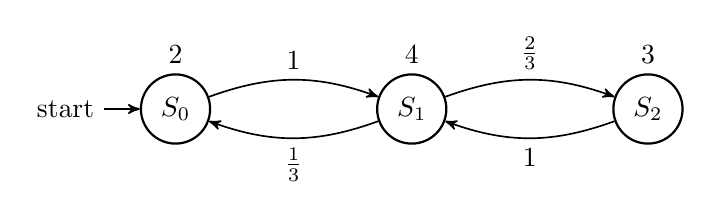
\begin{tikzpicture}[->, >=stealth', auto, semithick, node distance=3cm]
        \tikzstyle{every state}=[fill=white,draw=black,thick,text=black]
        \node[initial, state, label=above:2]    (S0)                   {$S_0$};
        \node[state, label=above:4]    (S1)[right of=S0]      {$S_1$};
        \node[state, label=above:3]    (S2)[right of=S1]      {$S_2$};
        \path

        (S0)
        edge [bend left=20] node{$1$} (S1)

        (S1)
        edge [bend left=20] node{$\frac{2}{3}$} (S2)
        edge [bend left=20] node{$\frac{1}{3}$} (S0)

        (S2)
        edge [bend left=20] node{$1$} (S1);
    \end{tikzpicture}
    \caption{An example of a CTMC with 3 states.}
    \label{fig:ctmc}
\end{figure}
Continous-time Markov chain has a wide range of applications, especially in bioinformatics where
chemical reaction network \cite{feinberg1980chemical} \cite{anderson2011continuous}. However, the
frameworks in this thesis apply for discrete-time Markov models, thus we do not use continuous-time
Markov chain to model systems of interest directly. Instead, we do not use Continuous-time Markov
models directly. Instead, we transform CTMCs into DTMCs through uniformization \cite{katoen2016probabilistic}
\begin{definition}[CTMC Uniformization]
    abcd
\end{definition}

\begin{figure}[H]
    \centering
    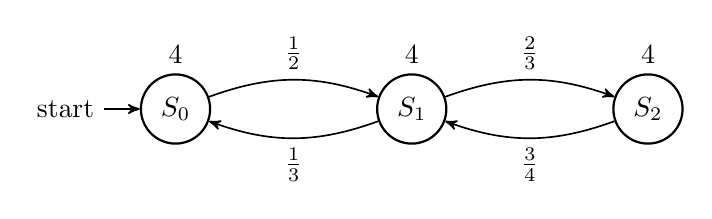
\begin{tikzpicture}[->, >=stealth', auto, semithick, node distance=3cm]
        \tikzstyle{every state}=[fill=white,draw=black,thick,text=black]
        \node[initial, state, label=above:4]    (S0)                   {$S_0$};
        \node[state, label=above:4]    (S1)[right of=S0]      {$S_1$};
        \node[state, label=above:4]    (S2)[right of=S1]      {$S_2$};
        \path

        (S0)
        edge [bend left=20] node{$\frac{1}{2}$} (S1)

        (S1)
        edge [bend left=20] node{$\frac{2}{3}$} (S2)
        edge [bend left=20] node{$\frac{1}{3}$} (S0)

        (S2)
        edge [bend left=20] node{$\frac{3}{4}$} (S1);
    \end{tikzpicture}
    \caption{The uniformized  CTMC of \ref{fig:ctmc}.}
\end{figure}
It has been shown by Katoen \cite{katoen2013model} that uniformization preserves the transient
probability distributions. Furthermore, in this thesis we concern steady state data and state
property, thus uniformizing exit rate does not affect the validity of our constructed frameworks.

\section{Probabilistic temporal logic}
We define the set of PCTL properties,
\begin{definition}[PCTL] The syntax of PCTL consists of state formulas and path formulas.
    \begin{itemize}
        \item State formulas
              \begin{align*}
                  \Phi & ::== \text{true} \;|\; a \;|\; \Phi \;|\; \Phi \wedge \Phi \;|\; \Phi \vee \Phi \;|\;  P_{\sim  p}[\phi]
              \end{align*}
        \item Path formulas
              \begin{align*}
                  \phi & ::== \bigcirc \Phi \;|\; \Phi \mathsf{U}  \Phi
              \end{align*}
    \end{itemize}

\end{definition}

\subsection{Model checking PCTL properties}
Given a DTMC $\mathcal{M}$ and a PCTL property $\Phi$, general algorithm for checking
$\mathcal{M}\models\Phi$ is described as following:

%% Argues the complexity
\subsection{State exlosion problem}


\section{Statistical Model checking}
Statistical model checking is a simulation-based approach to model check a stochastic model
$\mathcal{M}$ against a temporal property $\Phi$. The essential concept of probabilistic model
checking is to simulate traces from $\mathcal{M}$, verify if each trace satisfies $\Phi$, then
estimate probability $P(\mathcal{M}\models\Phi)$ by a statistical, frequentist approach.
\subsection{Statistical model checking of unbounded properties.}
Estimation method, Chernoff-Hoeffding bound.


\subsection{Statistical model checking of bounded properties.}
%% 

\section{Parametric model}
We introduce parameters to formalize unknown attributes of the system.
\begin{definition}[Polynomial ring]
    Given a tuple $\mathbf{x}=(x_1,\ldots,x_n)$ be a tuple
\end{definition}

\begin{definition}{Rational functions}
    Let $\mathbf{x}=\{x_1,\ldots,x_n\}$ be a variable; let $\mathbf{Pol}[\mathbf{x}]$ be the set of
    all polynomial functions over $\mathbf{x}$. A rational function $h(\mathbf{x})$ is defined
    as following.
    \begin{align*}
        h(x) := \frac{f(\mathbf{x})}{g(\mathbf{x})}, f,g\in\mathbf{Pol}[\mathbf{x}], g(\mathbf{x}) \neq 0
    \end{align*}
    We denote $\mathbb{Q}(\mathbf{x})$ the set of all rational functions over $\mathbf{x}$.
\end{definition}


\subsection{Parametric Discrete Time Markov chain}
With the set of rational functions formally defined, we define parametric Discrete-time Markov chain
based the definition on \cite{junges2019parameter}.
\begin{definition}[Discrete Time Markov Chain]
    A Discrete-time Markov chain (DTMC) is a tuple $(S, \mathbf{x}, \mathbf{P}, \iota_{init}, AP, L)$
    where
    \begin{itemize}
        \item $S$ is a countable, non-emty set of \textit{states}
        \item $\mathbf{x} \in \mathbb{R}^n, n \in \mathbb{N}$ as the set of $n$ real parameters.
        \item $\mathbf{P}:S\times S \rightarrow \mathbb{Q}(\mathbf{x})$ is the \textit{transition
                  probability} function such that
              \begin{align*}
                  \forall s \in S : \sum_{s'\in S}\mathbf{P}(s, s') = 1
              \end{align*}
        \item $\iota_{init}: S \rightarrow [0,1]$ is the \textit{initial distribution} such that
              \begin{align*}
                  \sum_{s\in S}\iota_{init}(s) = 1
              \end{align*}
        \item $AP$ is a set of \textit{atomic propositions}
        \item $L: S \rightarrow 2^{AP}$ is the labelling function on states.
    \end{itemize}
\end{definition}

\begin{example}[Parametric Knuth-Yao die]
    \begin{figure}[H]
        \centering
        \includegraphics[width=0.5\textwidth]{figures/knuth_die_pq.png}
        \caption{Knuth-Yao die to simulate a 6-faced die by two unfair coins with probability of one
            side $p$ and $q$. Image taken from \cite{katoen2016probabilistic}.}
    \end{figure}
\end{example}

Given a parametric Discrete-time Markov chain $\mathcal{M}_\theta$. A concrete assignment of parameter $\theta$
\textit{instantiates} a non-parametric Discrete-time Markov chain if $f{\theta}$ evaluates to a
real value for all $f\in\mathbf{P}$.

\subsection{Symbolic model checking of pDTMC}

\begin{example}{Parametric Knuth's die}
    We continue the example with Knuth die model $\mathcal{M}_{p}$. Assume the
    \begin{align*}
        x =
    \end{align*}
\end{example}

\subsection{Parameter synthesis of pDTMC}

\begin{example}
    Given a pDTMC of Knuth die $\mathcal{M}_{p}$ and a path property $\Phi = P_{\geq 0.2} [F
                \texttt{"one"}]$, synthesize parameter $p$ so that $\mathcal{M}_{p} \models \Phi$. A simple
    Monte-Carlo search on parameter space gives the following satisfying point:
    %% Figures
\end{example}
\section{Statistical Model checking}
Statistical model checking must be performed on an instantiated Markov chain.


\chapter{Bayesian inference}
We present essential concepts in Bayesian parameter inference and several methods to estimate
posterior distribution. The methods range from posterior conjugations, in which tractability is
guaranteed as we know the analytic form of both likelihood and prior distribution. Afterwards, we
discuss different sampling algorithm to approximate the posterior distribution when no conjugations
are available. We also present a likelihood-free method to exploit in the case that the analytical
form of the likelihood is not achievable or is too complex to evaluate. The sampling algorithms
presented in this chapter are the building block for the Bayesian frameworks that we present in this
thesis.

\section{Bayesian inference}
\subsection{Bayesian formula}
Let $D_{obs}$ be observed data. In statistical inference, we assume that the observed data has a
probability distribution of unknown parameter $\theta$, that is $D_{obs} \sim P(D_{obs}|\theta)$.
There are two main approaches in statistical inference: frequentist approach and Bayesian approach.
In the frequentist approach, the estimation of $\theta$ is based on long-run property, that is, given a
large enough sample size, expected value of parameter estimation $\hat{\theta}$ is equal to
$\theta$. Therefore, frequentist approach requires to gather a large amount of data to deliver a
close estimation $\hat{\theta}$.  The main advantage of Bayesian approach over frequentist approach
is that it require less data to obtain an estimation $\hat{\theta}$.\\
In Bayesian approach, we use the information gained from previously observed data \textit{(beliefs)}
to enhance the accuracy of the estimation of $\hat{\theta}$. The beliefs obtained from prior
knowledge of model parameter $\theta$ is represented by \textit{prior distribution} $\pi(\theta)$.
We have the \textit{likelihood} $P(D_{obs}|\theta)$ as the probability distribution over observed
data, given parameter $\theta$.
\begin{definition}[Bayes theorem]
    \rm
    \begin{align*}
        \pi(\theta | D_{obs}) = \frac{P(D_{obs}|\theta)\pi(\theta)}{\int_\theta P(D_{obs}|\theta)\pi(\theta)d\theta}
    \end{align*}
    where
    \begin{itemize}
        \item $\pi(\theta)$ is the \textit{prior distribution}.
        \item $P(D_{obs}|\theta)$ is the \textit{likelihood}.
        \item $\int_\theta P(D_{obs}|\theta)\pi(\theta)d\theta$ is the \textit{marginal distribution}.
        \item $\pi(\theta | D_{obs})$ is the \textit{posterior distribution}
    \end{itemize}
\end{definition}
The essential part of Bayesian inference in statistic is to compute or estimate the posterior
distribution. From the analytical form or the samples from the posterior distribution, we estimate
the model parameter $\theta$.

\subsection{Bayesian parameter estimation}
With posterior distribution $\pi(\theta|D_{obs})$ we estimate the parameter $\hat{\theta}$ using Bayesian
posterior mean.
\begin{definition}[Bayesian posterior mean]
    \rm
    \begin{align*}
        \hat{\theta} = \mathbf{E}[\theta] = \int_\theta \theta \pi(\theta|D_{obs}) d\theta
    \end{align*}
\end{definition}
In case we have samples from posterior distribution, for example a trace of $N$ parameter values
$(\theta_1,\ldots,\theta_N)$ sampled from the posterior distribution $\pi(\theta|D_{obs})$, the
discrete form of posterior mean is used:
\begin{align*}
    \hat{\theta} \approx \mathbf{E}[\theta] \approx \sum_\theta \theta \pi(\theta|D_{obs})
\end{align*}

\begin{definition}[Bayesian Credible Set]
    Set C is a $(1 − \alpha )100\%$ credible set for the parameter $\theta$ if the posterior
    probability for $\theta$ to belong to C equals $(1 − \alpha)$.
    \begin{align*}
        P(\theta \in C | D_{obs}) = \int_C \pi(\theta|D_{obs}) d\theta = 1 - \alpha
    \end{align*}
\end{definition}
In this thesis, we use by default $0.95$ credible set, which corresponds to $\alpha=0.05$
\begin{definition}[Highest Posterior Density credible set]
    Highest Posterior Density $(1-\alpha)100\%$ credible set (HPD for short) is the
    interval with minimum length over all Bayesian $(1-\alpha)100\%$ Credible Set.
\end{definition}

In this research, the HPD is calculated using algorithm from \textit{PyMC3} library
\cite{salvatier2016pymc3}. For simplicity, we assume that in all cases which we concern, HPD is
computed using the algorithm for unimodal distribution.
\begin{algorithm}[H]
    \footnotesize{
        \hspace*{\algorithmicindent} \textbf{Input:}
        \begin{itemize}[noitemsep,topsep=0pt]
            \item $S$: is samples from a distribution.
            \item $0\leq \alpha \leq 1$: confidence level.
        \end{itemize}
        \hspace*{\algorithmicindent} \textbf{Output:} HPD interval.
    }
    \begin{algorithmic}[1]
        \Procedure{Compute HPD}{$S$}
        \State Compute interval width $w = |S| * \alpha$
        \State Find modal (peak) of sample points.
        \State Return minimal interval of size $|S| - w$ which contains the modal.
        \EndProcedure
    \end{algorithmic}
    \caption{Compute Highest Posterior Density Interval}
    \label{alg:hpd}
\end{algorithm}

\subsection{Selection of prior distribution}
Theoretically in Bayesian inference, prior distribution can be of any distribution family. However,
a selection of prior distribution that is too different than the actual distribution of parameter
can leads to a false propagation of beliefs and degrade the inference results. It is suggested by
\cite{polgreen2016data} that in case of no prior knowledge exists, Uniform distribution is
preferable since it is less likely to propagate false beliefs to the inference. In this thesis, we
use uniform distribution as the prior distribution on model parameters.

\subsection{Estimation of posterior distribution}
\subsubsection{Posterior conjugation}
Conjugated posteriors are special cases of Bayesian inference, in which the prior and posterior
distribution belongs to the same family of distribution. When posterior conjugation is applicable,
only the parameters of probability distribution function need to be re-estimated. Applying
conjugated posterior when it is possible gives advantages:
\begin{itemize}
    \item Tractability: we have analytical form of posterior distribution with only changes in its
          parameters.
    \item Computationally effective: updating model parameter is of linear time to the dimension of
          parameter.
\end{itemize}
We consider two conjugated posteriors as examples: Binomial-Beta and Dirichlet-Multinomial.
\begin{lemma}[Binomial-Beta Conjugation]
    Binomial distribution is conjugated to beta distribution.
\end{lemma}
\begin{proof}
    The observed data $D=(x_1,\ldots,x_n)$ is sampled from $Binomial(k, \theta)$ function
    \begin{align*}
        P(D|\theta) = \prod_{i=1}^n{k\choose x_i}\theta^{x_i}(1-\theta)^{k-x_i}
    \end{align*}
    The parameter $\theta$ is of $Beta(\alpha, \beta)$ distribution
    \begin{align*}
        \pi(\theta) = \theta^{\alpha-1}(1-\theta)^{\beta -1}
    \end{align*}
    We obtained:
    \begin{align*}
        \pi(\theta|D) & \sim P(D|\theta)\pi(\theta)                                                                             \\
                      & \sim \theta^{\sum_{i=1}^n x_i}(1-\theta)^{nk -\sum_{i=1}^n x_i} \theta^{\alpha -1} (1-\theta)^{\beta-1} \\
                      & = \theta^{\alpha - 1 + \sum_{i=1}^n x_i}(1-\theta)^{\beta - 1 + nk -\sum_{i=1}^n x_i}
    \end{align*}
    Thus, the posterior is $Beta(\alpha + \sum_{i=1}^n x_i, \beta + nk -\sum_{i=1}^n x_i)$
\end{proof}
Generalize this conjugation, we also have Multinomial-Dirichlet conjugation.
\begin{lemma}[Multinomial-Dirichlet Conjugation]
    Multinomial distribution is conjugated to Dirichlet distribution.
\end{lemma}
\begin{proof}
    The observed data $D=(x_1,\ldots,x_n)$ is sampled from $Multinomial(n; \theta_1,\ldots,\theta_n)$ function
    \begin{align*}
        P(x_1,\ldots,x_n | N, \theta_0,\ldots,\theta_n) & = \frac{n!}{x_1!\ldots x_n!} \prod_{i=1}^n\theta_i^{x_i}
    \end{align*}
    The parameter $(\theta_1,\ldots,\theta_n)$ is
    $Dirichlet(\alpha_1,\ldots,\alpha_n)$
    \begin{align*}
        \pi(\theta_1,\ldots,\theta_n) = \frac{1}{\mathbf{B}(\alpha_1,\ldots,\alpha_n)}\prod_{i=1}^n\theta_i^{\alpha_i - 1}
    \end{align*}
    We obtain
    \begin{align*}
        \pi(\theta_1,\ldots,\theta_n|D) & \sim P(D|\theta)\pi(\theta)                                           \\
                                        & \sim \prod_{i=1}^n\theta_i^{x_i} \prod_{i=1}^n\theta_i^{\alpha_i - 1} \\
                                        & \sim \prod_{i=1}^n\theta_i^{\alpha_i - 1 + \sum_{i=1}^n x_i}
    \end{align*}
    Thus, the posterior is $Dirichlet(\alpha_1 +  x_1,\ldots,\alpha_n
        +  x_n)$
\end{proof}
More detailed description in these cases can be found in \cite{tu2014dirichlet}
and \cite{baron2019probability}. We summarize the necessary results in the following table:
\begin{table}[H]
    \begin{tabular}{lllll}
        \cline{1-3}
        \multicolumn{1}{|l|}{Likelihood}                                 & \multicolumn{1}{l|}{Prior}                                 & \multicolumn{1}{l|}{Posterior parameters}                         &  & \\ \cline{1-3}
        \multicolumn{1}{|l|}{$Binomial(n, k)$}                           & \multicolumn{1}{l|}{$Beta(\alpha, \beta)$}                 & \multicolumn{1}{l|}{\begin{tabular}[x]{@{}c@{}}$\alpha' = \alpha + \sum_{i=1}^n x_i$\\$\beta' = \beta + nk -\sum_{i=1}^n x_i$\end{tabular}}                   &  & \\ \cline{1-3}
        \multicolumn{1}{|l|}{$Multinomial(n; \theta_1,\ldots,\theta_n)$} & \multicolumn{1}{l|}{$Dirichlet(\alpha_1,\ldots,\alpha_n)$} & \multicolumn{1}{l|}{$\alpha_i' =\alpha_i + x_i, 1 \leq i \leq n$} &  & \\ \cline{1-3}
                                                                         &                                                            &                                                                   &  &
    \end{tabular}
\end{table}
However, posterior conjugation is applicable to a subset of prior and likelihood functions. In
Bayesian inference, it is common that the posterior distribution has no analytical form or its
analytical form is difficult to directly sample from. In these cases, we can several different
sampling and optimization methods to approximate the posterior distribution. In the following
section we discuss different approaches for posterior distribution approximation:
\begin{itemize}
    \item Markov chain Monte Carlo.
    \item Sequential Monte Carlo.
    \item Approximate Bayesian Computation.
\end{itemize}

\subsubsection{Markov chain Monte Carlo}
In case the posterior distribution has no analytical form or its analytical form is difficult to
sample from directly, we use \textit{Metropolis-Hastings} algorithm  (\textit{MH} in short). Firstly
introduced by Metropolis \cite{metropolis1953equation} and later generalized by Hastings
\cite{hastings1970monte} Metropolis-Hastings algorithm is a \textit{Monte Carlo Markov Chain}
algorithm. In its essential, Metropolis-Hastings algorithm draws sample from an unknown
distribution. Using the MH algorithm, we can estimate the parameter by posterior mean, without
knowing the analytical form of posterior distribution itself. A special case of MH algorithm is
Gibbs sampling algorithm \cite{geman1984stochastic}, in which candidates are accepted with
probability 1. Gibbs sampling can be used to draw samples from multivariate posteriors when the
parameter is of high dimensional. Quality of data can also impacts the estimation result from
Metropolis-Hastings algorithm; in case of experiment data is acquired from a small sample size,
statistical techniques to improve data quality can be used, for example \textit{bootstrapping}
\cite{efron1992bootstrap}.

\begin{algorithm}[H]
    \caption{Metropolis-Hastings Algorithm}
    \label{alg:mh}
    \footnotesize{
        \hspace*{\algorithmicindent} \textbf{Input:}
        \begin{itemize}[noitemsep,topsep=0pt]
            \item Model $\mathcal{M}_\theta$
            \item $D_{obs}$: observation data
            \item $P(D|\theta)$: likelihood function
            \item $\pi(\theta)$: prior distribution
            \item Transition kernel $Q(\theta^t|\theta^{t-1})$
            \item $N$ number of particles.
        \end{itemize}
        \hspace*{\algorithmicindent} \textbf{Output:}
        \begin{itemize}[noitemsep,topsep=0pt]
            \item $(\theta_1,\ldots,\theta_N)$ sample of $N$ particles
            \item $(w_1,\ldots,w_N)$ corresponding likelihoods.
        \end{itemize}
    }
    \begin{algorithmic}[1]
        \Procedure{Metropolis-Hastings}{}
        \State Draw $\theta_{cand}$ from $\pi(\theta)$
        \State $\theta_1 \leftarrow  \theta_{cand}$
        \State $w_1 \leftarrow  \ln(P(D_{obs}|\theta_{cand}))$
        \State $i \leftarrow 2$
        \While{$i \leq N_{MH}$}
        \State Draw $\theta_{cand}$ from $Q(\theta'|\theta_{i-1})$
        \If{ $\ln(P(D_{obs}|\theta_{cand})) - \ln(P(D_{obs}|\theta_{i-1})) > 0$ }
        \State $\theta_i \leftarrow \theta_{cand}$
        \State $w_i \leftarrow \ln(P(D_{obs}|\theta_{cand}))$
        \State $i \leftarrow i + 1$
        \Else
        \State Draw a random number $u$ from $Uniform(0,1)$
        \If{$u \leq \xi$, ($\xi$ small, e.g $10^{-2}$)}
        \State $\theta_i \leftarrow \theta_{cand}$
        \State $w_i \leftarrow \ln(P(D_{obs}|\theta_{cand}))$
        \State $i \leftarrow i + 1$
        \EndIf
        \EndIf
        \EndWhile
        \State Return $(\theta_1,\ldots,\theta_{N}})$, $(w_1,\ldots,w_{N}})$
        \EndProcedure
    \end{algorithmic}
\end{algorithm}

The likelihood function can be implemented as log-likelihood to avoid underflow error.
Advantages of Metropolis-Hastings are:
\begin{itemize}
    \item[+] Parameter transition only needs the computation of likelihood function.
          Therefore, Monte Carlo Markov Chain can be used in general Bayesian inference,
          in which we are not guaranteed to have an analytical form of posterior.
    \item[+] Computationally efficient; as marginal distribution is cancelled out, and likelihood can
          be replaced by log-likelihood, Metropolis-Hastings simplifies the computation of Bayes formula
          and avoid infinitesimal values.
    \item[+] Simple to implement.
\end{itemize}
Disadvantages of Metropolis-Hastings are
\begin{enumerate}
    \item[-] Particle in Metropolis-Hastings algorithm moves in a linear Markov chain; it is highly
          probable to be stuck in a local maximum or minimum.
    \item[-] Not parallelizable; since there is only one linear chain, and current step depends on
          previous step, Metropolis-Hastings algorithm does not scale up to multi-processors.
\end{enumerate}
The next algorithm, \textit{Sequential Monte Carlo}, addresses the issues of Metropolis-Hastings.

\subsubsection{Sequential Monte Carlo}
Sequential Monte Carlo method is firstly proposed by Del \cite{del2006sequential}. Instead of having
one particle moving in its parameter space, Sequential Monte Carlo estimates by using $N$ particles
moving independently. In its initial step, Sequential Monte Carlo draws a parameter candidate from
the prior distribution. In each iteration, it then mutates parameter candidates through a series of
\textit{perturbation kernels} and select parameter candidates for the next iteration with regarding
to their weights. By sampling from $N$ independently moving particles, Sequential Monte Carlo method
has a significant advantage of easily parallelizable. Furthermore, Daviet \cite{daviet2018inference}
shows that Sequential Monte Carlo delivers better performance on approximating multimodal
distribution.

\begin{algorithm}[H]
    \caption{Sequential Monte Carlo Algorithm}
    \label{alg:smc}
    \footnotesize{
        \hspace*{\algorithmicindent} \textbf{Input:}
        \begin{itemize}[noitemsep]
            \item Model $\mathcal{M}_\theta$
            \item $D_{obs}$: observation data
            \item $\pi(\theta)$: prior distribution
            \item $P(D|\theta)$: Likelihood function.
            \item $Q(\theta^t|\theta^{t-1})$: Transition kernel.
            \item $F_t(\theta^t|\theta_1^{t-1},\ldots,\theta_N^{t-1})$: Perturbation kernels
            \item $N$ number of particles.
        \end{itemize}
        \hspace*{\algorithmicindent} \textbf{Output:}
        \begin{itemize}[noitemsep]
            \item $(\theta_1,\ldots,\theta_N)$ sample of $N$ particles
            \item $(w_1,\ldots,w_N)$ corresponding likelihoods.
        \end{itemize}
    }
    \begin{algorithmic}[1]
        \Procedure{Sequential-Monte Carlo}{}
        \State $i \leftarrow 1$
        \While{$i \leq N$} \algorithmiccomment {SMC initialization}
        \State Draw $\theta$ from $\pi(\theta)$
        \State $\theta_i \leftarrow \theta$
        \State $w_i \leftarrow P(D_{obs}|\theta_i)$
        \State $i \leftarrow i + 1$
        \EndWhile
        \State $t \leftarrow 1$
        \While{$t \leq M$}
        \State $i \leftarrow 1$ \algorithmiccomment{SMC correction step}
        \While{$i \leq N$}
        \State $w'_i \leftarrow \frac{w_i}{\sum_{i=1}^N w_i} $
        \EndWhile
        \State Sample with replacement $(\theta'_1,\ldots,\theta'_N)$ \algorithmiccomment{SMC selection step} \\\hspace{1.5cm} from $(\theta_1,\ldots,\theta_N)$ with probabilities $(w'_1,\ldots,w'_N)$
        \State $(\theta_1,\ldots,\theta_N) \leftarrow (\theta'_1,\ldots,\theta'_N)$
        \State $i \leftarrow 1$
        \While{$i \leq N$} \algorithmiccomment {SMC perturbation step}
        \State Draw $\hat{\theta}^t_i$ from $F_t(\theta^t | \theta^{t-1}_1,\ldots,\theta^{t-1}_N), 1\leq t \leq M$
        \State $(\theta^*_1,\ldots,\theta^*_{N_{MH}}), (w^*_1,\ldots,w^*_{N_{MH}}) \leftarrow Metropolis-Hastings(\hat{\theta}^t_i)$
        \State $\theta_i \leftarrow \theta^*_{N_{MH}}$
        \State $w_i \leftarrow w^*_{N_{MH}}$
        \EndWhile
        \EndWhile
        \State Return $(\theta_1,\ldots,\theta_{N})$, $(w_1,\ldots,w_{N})$
        \EndProcedure
    \end{algorithmic}
\end{algorithm}
Selection of kernel function for SMC is mentioned by Filippi \cite{filippi2013optimality}, and Silk \cite{silk2012optimizing}.\\
Advantages of Sequential Monte Carlo algorithm:
\begin{itemize}
    \item[+] Approximate multimodal distributions: since Sequential Monte Carlo consists of $N$
          particles moving independently and later selected with replacement, it is less likely to fall
          into a local maximum or minimum.
    \item[+] Parallelizable: Sequential Monte Carlo has trivially data-parallelism, in contrast to
          Metropolis-Hastings where no parallelization is possible.
\end{itemize}
However, Sequential Monte Carlo also has disadvantages:
\begin{itemize}
    \item[-] Selection of perturbation and transition kernel is not trivial.
    \item[-] More difficult to implement.
\end{itemize}

\subsubsection{Approximate Bayesian Computation}
The methods mentioned before are used with an assumption that the likelihood $P(D_{obs}|\theta)$ has
an analytical form; the analytical form can be evaluated without introducing computational burden.
However for situations in which the likelihood has no analytical form, or the analytical form is
expensive to be evaluated, we use a class of \textit{likelihood-free methods}. Likelihood-free
methods in Bayesian inference estimates the likelihood $P(D_{obs}|\theta)$, or replace it by other
measures. \textit{Approximate Bayesian Computation} (or \textit{ABC} in short)
\cite{toni2009approximate} is a widely used likelihood-free method for approximating posterior
distribution. Instead of estimating the likelihood $P(D|\theta)$ directly, we define a distance
measure $\delta(D_1, D_2)$ where $D_1$ and $D_2$ denote observable data. Given a parameter candidate
$\hat{\theta}$ that specifies a model $\mathcal{M}_\theta$. The ABC algorithm accepts $\hat{\theta}$
if a simulation run on $\mathcal{M}_\theta$ delivers observable data $D_{sim}$ such that
$\delta(D_{obs},D_{sim}) < \epsilon$, where $\epsilon\in\mathbf{R}_{\leq 0}$ is the distance
threshold.
\begin{algorithm}[H]
    \caption{Approximate Bayesian Computation}
    \label{alg:abc-reject}
    \footnotesize{
        \hspace*{\algorithmicindent} \textbf{Input:}
        \begin{itemize}[noitemsep,topsep=0pt]
            \item Model $\mathcal{M}_\theta$
            \item $D_{obs}$: observation data
            \item $\pi(\theta)$: prior distribution
            \item $\delta(D_{sim}, D_{obs})$: distance function between two set of data simulated by $\mathcal{M}_\theta$
            \item $epsilon$: distance threshold
            \item $N$ number of particles.
        \end{itemize}
        \hspace*{\algorithmicindent} \textbf{Output:}
        \begin{itemize}[noitemsep]
            \item $(\theta_1,\ldots,\theta_N)$: $N$ sampled particles.
            \item $(w_1,\ldots,w_N)$: corresponding weights of sampled particles.
        \end{itemize}
    }
    \begin{algorithmic}[1]
        \Procedure{Approximate-Bayesian-Computation}{}
        \State Select a proposal distribution $\pi(\theta)$
        \State $i \leftarrow 1$
        \While{$i \leq N$}
        \State Draw a random particle $\theta$ from $\pi(\theta)$
        \State Simulate data $D_{sim}$ from $\mathcal{M}_\theta$
        \If{$d = \delta(D_{sim}, D_{obs}) < \epsilon$}
        \State $\theta_i \leftarrow \theta$
        \State $w_i = d$
        \EndIf
        \EndWhile
        \State Return $(\theta_1,\ldots,\theta_N)$, $(w_1,\ldots,w_N)$
        \EndProcedure
    \end{algorithmic}
\end{algorithm}
Advantages of Approximate Bayesian Computation:
\begin{itemize}
    \item[+] Likelihood-free: applicable when the likelihood has no analytical form or there is no likelihood.
    \item[+] Easy to implement.
\end{itemize}
Disavantages of Approximate Bayesian Computation:
\begin{itemize}
    \item[-] Which distances are proper to measure two data set? In the other word, is measuring
          distance a proper method to approximate likelihood?
    \item[-] How to select a threshold so that the likelihood is closely approximated?
\end{itemize}

\section{Summary}
We introduced basic concepts on Bayesian parameter inference and posterior estimation. Since the
posterior distributions normally have no analytical form, the presented sampling and
optimization methods which are essentials to posterior estimation. In the following chapter we
propose a data-driven approach for parameter synthesis combining Approximate Bayesian computation,
Sequential Monte Carlo, and Statistical Model Checking.

\chapter{Framework for parameter synthesis.}
\section{Model construction}


\section{Framework}


\chapter{Case studies}
To evaluate the effectiveness of the presented frameworks, we use three case studies. In each case
study, we benchmark the frameworks using the following steps:
\begin{enumerate}
    \item Describe the system of interest.
    \item Construct state-space and parametric transitions function for pDTMC models.
    \item Apply the frameworks in different setups (rational functions available, simulation-based)
          using synthetic data from known model parameters.
    \item Visualize the parameter synthesis and inference result.
    \item Measure runtime among different state-space to evaluate the frameworks' scalability.
\end{enumerate}
Three case studies include firstly a simple and standard case study \textit{zeroconf}. The second
case study comes from the experiments of the Department of Biology at the University of Konstanz on
the defensive behaviour of bee colonies\cite{hajnal2019data}. Third case study is an epidemics
model; it is introduced in order to show the expansion of the model state-space as the system has
more states to be encoded.

%%%%%%%%%%%%%%%%%%%%%%%%%%%%%%%%%%%%%%%%%%%%%%%%%%%%%%%%%%%%%%%%%%%%%%%%%%%%%%%%%%%%%%%%%%%%%%%%%%%

\section{Zeroconf}
Zero-configuration protocol (\textit{zeroconf} for short) is a protocol used in IPv4 network to
allocate newly attached device an unique IP address without any intervention from network operators.

\subsection{Model and properties}
From the pseudocode of Zeroconf protocol
\subsection{Evaluation}
\subsection{Summary}

%%%%%%%%%%%%%%%%%%%%%%%%%%%%%%%%%%%%%%%%%%%%%%%%%%%%%%%%%%%%%%%%%%%%%%%%%%%%%%%%%%%%%%%%%%%%%%%%%%%
\section{Bees colony}
\subsection{System description}
We study the collective behavior of a bee colony. Each bee in a colony possibly stings after
observing a threat in the surrounding environment, and warn other bees by releasing a special
substance, pheromone. By sensing the pheromone released in the environment, other bees in the colony
may also sting. However, since stinging leads to the termination of an individual bee, it reduces
the total defense capability as well. With parametric Discrete-time Markov chain as the model, we
study how the actions of a single bee change with regarding to the colony size of and pheromone
amount.

\subsection{Model and properties}
Assume that each bee in a colony decides its next action (to sting or not to sting) based only on
the current state of the environment, and the number of bees who sting or not sting can be modeled
as a Markov process. To reduce the complexity of the model, we make another assumption that the
states of the bees colony are observed after uniform time duration, hence the model is of
discrete-time.There are 3 assumptions on the system:
\begin{enumerate}
    \item Each bee release an unit amount of pheromone immediately after stinging.
    \item A bee dies after stinging and releasing pheromone. In the other words, no bee can sting
          more than once.
    \item Stinging behaviour only depends on the concentration of pheromone in the environment.
\end{enumerate}
Under these assumption, a bee colony can be viewed as a set of agents (bees) interact with each
other in a closed environment with the appearance of a factor \textit{pheromone}. Afterward, the
agent has probability to commit an action, namely \textit{sting}. The agent is eliminated from
environment after stinging. Assume that we have a colony of $n$ bees initially. As aforementioned,
an individual bee is terminated after it stings. Thus, at the end of experiment, the number of bees
is $n'\in\{0,1,\ldots,n\}$. We model the bee colony with a DTMC $\mathcal{M}=(S,\mathbf{P},
    S_{init}, AP,L)$, such that
\begin{itemize}
    \item $|S_{init}|=1$
    \item There exists $n+1$ tSCCs which encode the population at the end of the experiment.
\end{itemize}

\begin{figure}[H]
    \centering
    \begin{tikzpicture}[->, >=stealth', auto, semithick, node distance=4cm]
        \tikzstyle{every state}=[fill=white,draw=black,thick,text=black]
        \node[state]    (A)                     {init};
        \node[state,accepting]    (D)[right of=A]         {$1,1,1$};
        \node[state]    (C)[below of=D]         {$0,1,1$};
        \node[state]    (B)[above of=D]         {$0,0,1$};
        \node[state]    (E)[left of=A]          {$0,0,0$};

        \node[state]    (F)[right of=D]         {$1,-1,-1$};
        \node[state]    (G)[above of=B]         {$1,1,-1$};

        \node[state]    (H)[below of=F]         {$1,1,-2$};
        \path
        (A)
        edge    node{$3r_0(1-r_0)^2$}      (B)
        edge    node{$3r_0^2(1-r_0)$}      (C)
        edge    node{$r_0^3$}              (D)
        edge    node{$(1-r_0)^3$}          (E)

        (B)
        edge    node{$(1-\frac{r_1-r_0}{1-r_0})^2$}                                  (F)
        edge    node{$2\frac{1-r_0}{r_1-r_0}(1-\frac{r_1-r_0}{1-r_0})$}              (G)
        edge    node{$(\frac{r_1-r_0}{1-r_0})^2$}                                    (D)

        (C)
        edge    node{$1-\frac{r_2-r_0}{1-r_1}$}          (H)
        edge    node{$\frac{r_2-r_0}{1-r_1}$}            (D)

        (F)
        edge    node{$1-\frac{r_2-r_0}{1-r_1}$}          (H)
        edge    node{$\frac{r_2-r_0}{1-r_1}$}            (D);
    \end{tikzpicture}
    \caption{Synchronous model of 3 bees, multiparameters}
\end{figure}


Semantics of Markov population models for bees colony are developed by \cite{hajnal2019data}.
\subsection{Evaluation}
\subsection{Conclusion}

%%%%%%%%%%%%%%%%%%%%%%%%%%%%%%%%%%%%%%%%%%%%%%%%%%%%%%%%%%%%%%%%%%%%%%%%%%%%%%%%%%%%%%%%%%%%%%%%%%%
\section{SIR model}
\subsection{System}
\textit{SIR} model  is a population model, which is widely used in
modeling epidemics. In a \text{SIR} model, each individual is of one
among three types:
\begin{itemize}
    \item \textit{Susceptible (S)}
    \item \textit{Infected (S)}
    \item \textit{Recovered (S)}
\end{itemize}
SIR system is a stochastic system modeled by reactions between S, I and R. In this thesis we use only 2 reactions.
\begin{equation*}
    S + I \xrightarrow{\alpha} 2I \\
    I \xrightarrow{\beta} R
    \label{eqn:sir}
\end{equation*}

\begin{algorithm}[H]
    \caption{Generate SIR CTMC from reactions.}
    \label{alg:gen-sir-ctmc}
    \hspace*{\algorithmicindent} \textbf{Input:}
    \begin{itemize}
        \item $(S_0, I_0, R_0)$: initial population.
        \item Reactions of rate $\alpha,\beta$
              \begin{equation*}
                  S + I \xrightarrow{\alpha} 2I \\
                  I \xrightarrow{\beta} R
              \end{equation*}
    \end{itemize}
    \hspace*{\algorithmicindent} \textbf{Output:}
    \begin{itemize}
        \item CTMC $\mathcal{C}$
    \end{itemize}
    \begin{algorithmic}[1]
        \Procedure{Sir-Explore-Statespace}{}
        \If{$i = 0$}
        \EndIf
        \If{$(s>0) \wedge (i>0)$}
        \State Sir-Explore-Statespace
        \EndIf
        \If{$(i>0)$}
        \State Sir-Explore-Statespace
        \EndIf
        \EndProcedure
        \Procedure{Sir-Explore-Statespace}{}
        \If{$i = 0$}
        \EndIf
        \If{$(s>0) \wedge (i>0)$}
        \State Sir-Explore-Statespace
        \EndIf
        \If{$(i>0)$}
        \State Sir-Explore-Statespace
        \EndIf
        \EndProcedure
    \end{algorithmic}

\end{algorithm}

\subsection{Model and properties}

\begin{theorem}{Acyclicity}
    A CTMC $\mathcal{C}$ constructed by Algorithm \ref{alg:gen-sir-ctmc} using reactions
    \ref{eqn:sr} is acyclic.
\end{theorem}
\textbf{Proof}: For any arbitrary transition in $\mathcal{C}$
\begin{enumerate}
    \item $|S|$ is monotonically decreasing, as there exists no reaction which produces $S$.
    \item $|R|$ is monotonically increasing, as there exists no reaction which consumes $R$.
    \item If $P((s,i,r), (s',i',r'))\neq 0$, then $i \neq i'$. That is because all reactions change $i$.
\end{enumerate}
As $|S| + |I| + |R| = S_0 + I_0 + R_0$ and $S_0,R_0,I_0$ are constants, if there exists a path fragment
\begin{align*}
    (s^t,i^t,r^t)\rightarrow \quad \ldots \quad \rightarrow(s^{t+k},i^{t+k},r^{t+k})
\end{align*}
such that $(s^t,i^t,r^t) = (s^{t+k},i^{t+k},r^{t+k})$ then $k=0$, because all reactions change $i$
(if $P((s,i,r), (s',i',r'))\neq 0$, then $i \neq i'$). \QED
\begin{corollary}
    A CTMC constructed by Algorithm \ref{alg:gen-sir-ctmc} using reactions \ref{eqn:sr} has BSCCs
    and the BSCCs are trivial.
\end{corollary}

\begin{example}
    Example of an SIR CTMC model with initial population $(S_0, I_0, R_0) = (3,1,0)$
    \begin{figure}[H]
        \centering
        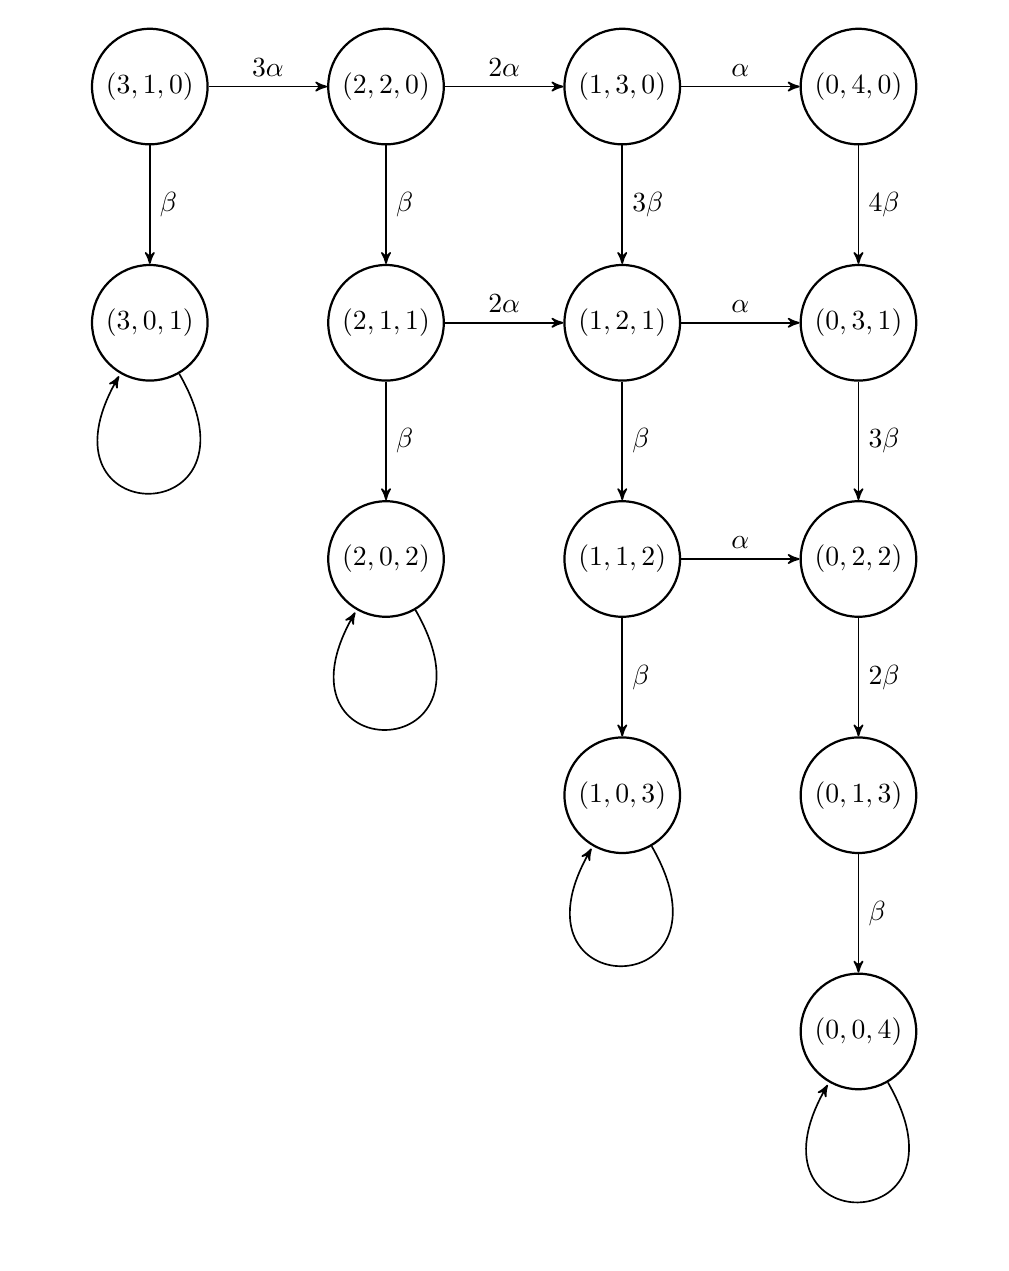
\begin{tikzpicture}[->, >=stealth', auto, semithick, node distance=3cm]
            \tikzstyle{every state}=[fill=white,draw=black,thick,text=black]
            \node[state]    (Init)                      {$(3,1,0)$};
            \node[state]    (S_301)[below of=Init]      {$(3,0,1)$};
            \node[state]    (S_220)[right of=Init]      {$(2,2,0)$};
            \node[state]    (S_211)[below of=S_220]     {$(2,1,1)$};
            \node[state]    (S_202)[below of=S_211]     {$(2,0,2)$};
            \node[state]    (S_130)[right of=S_220]     {$(1,3,0)$};
            \node[state]    (S_121)[below of=S_130]     {$(1,2,1)$};
            \node[state]    (S_112)[below of=S_121]     {$(1,1,2)$};
            \node[state]    (S_103)[below of=S_112]     {$(1,0,3)$};
            \node[state]    (S_040)[right of=S_130]     {$(0,4,0)$};
            \node[state]    (S_031)[below of=S_040]     {$(0,3,1)$};
            \node[state]    (S_022)[below of=S_031]     {$(0,2,2)$};
            \node[state]    (S_013)[below of=S_022]     {$(0,1,3)$};
            \node[state]    (S_004)[below of=S_013]     {$(0,0,4)$};
            \path
            (Init)
            edge node{$\beta$} (S_301)
            edge node{$3\alpha$} (S_220)

            (S_220)
            edge node{$2\alpha$} (S_130)
            edge node{$\beta$} (S_211)

            (S_130)
            edge node{$\alpha$} (S_040)
            edge node{$3\beta$} (S_121)

            (S_040)
            edge node{$4\beta$} (S_031)

            (S_031)
            edge node{$3\beta$} (S_022)

            (S_022)
            edge node{$2\beta$} (S_013)

            (S_013)
            edge node{$\beta$} (S_004)

            (S_121)
            edge node{$\alpha$} (S_031)
            edge node{$\beta$} (S_112)

            (S_112)
            edge node{$\alpha$} (S_022)
            edge node{$\beta$} (S_103)

            (S_211)
            edge node{$2\alpha$} (S_121)
            edge node{$\beta$} (S_202)

            (S_301)
            edge [in=240,out=300,loop]  ()

            (S_202)
            edge [in=240,out=300,loop]  ()

            (S_103)
            edge [in=240,out=300,loop]  ()

            (S_004)
            edge [in=240,out=300,loop]  ();

        \end{tikzpicture}
        \caption{$SIR(3,1,0)$ CTMC model with parameters$(\alpha, \beta)$}
    \end{figure}
\end{example}

\begin{example}
    Uniformize the chain with uniformization rate $(3\alpha + 4\beta)$, we derive the following uniformized DTMC:
    \begin{figure}[H]
        \centering
        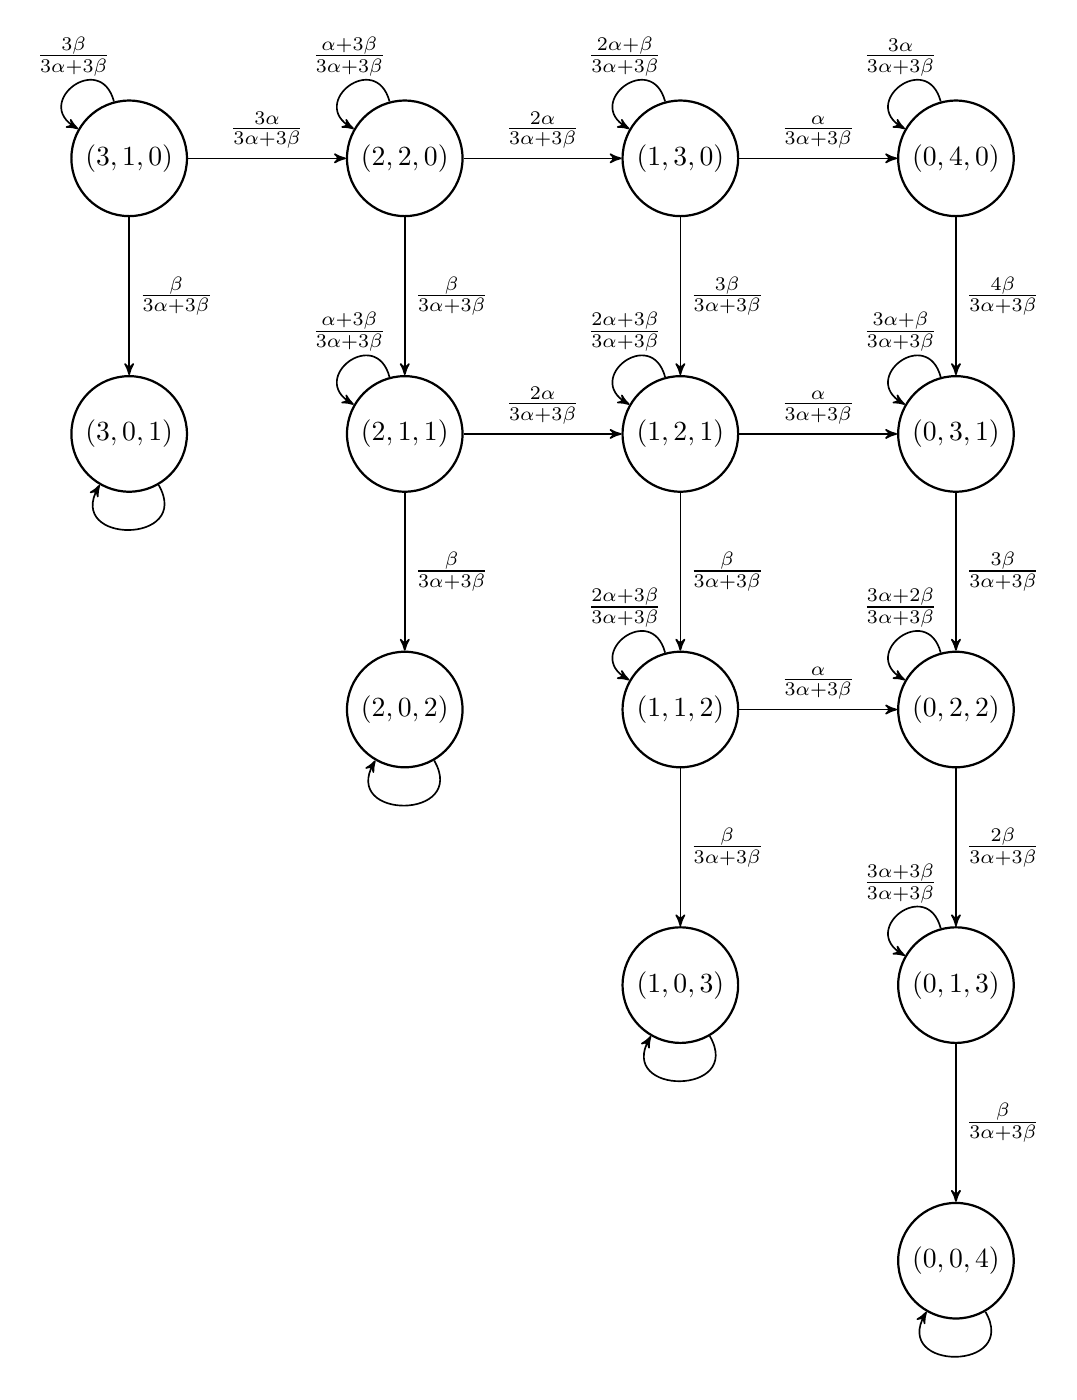
\begin{tikzpicture}[->, >=stealth', auto, semithick, node distance=3.5cm]
            \tikzstyle{every state}=[fill=white,draw=black,thick,text=black]
            \node[state]    (Init)                      {$(3,1,0)$};
            \node[state]    (S_301)[below of=Init]      {$(3,0,1)$};
            \node[state]    (S_220)[right of=Init]      {$(2,2,0)$};
            \node[state]    (S_211)[below of=S_220]     {$(2,1,1)$};
            \node[state]    (S_202)[below of=S_211]     {$(2,0,2)$};
            \node[state]    (S_130)[right of=S_220]     {$(1,3,0)$};
            \node[state]    (S_121)[below of=S_130]     {$(1,2,1)$};
            \node[state]    (S_112)[below of=S_121]     {$(1,1,2)$};
            \node[state]    (S_103)[below of=S_112]     {$(1,0,3)$};
            \node[state]    (S_040)[right of=S_130]     {$(0,4,0)$};
            \node[state]    (S_031)[below of=S_040]     {$(0,3,1)$};
            \node[state]    (S_022)[below of=S_031]     {$(0,2,2)$};
            \node[state]    (S_013)[below of=S_022]     {$(0,1,3)$};
            \node[state]    (S_004)[below of=S_013]     {$(0,0,4)$};
            \path[->, every loop/.style={looseness=3}]
            (Init)
            edge node{$\frac{\beta}{3\alpha + 3\beta}$}   (S_301)
            edge node{$\frac{3\alpha}{3\alpha + 3\beta}$} (S_220)
            edge[in=150,out=105,loop] node[above]{$\frac{3\beta}{3\alpha + 3\beta}$} ()

            (S_220)
            edge node{$\frac{2\alpha}{3\alpha + 3\beta}$} (S_130)
            edge node{$\frac{\beta}{3\alpha + 3\beta}$} (S_211)
            edge[in=150,out=105,loop] node[above]{$\frac{\alpha+3\beta}{3\alpha + 3\beta}$} ()

            (S_130)
            edge node{$\frac{\alpha}{3\alpha + 3\beta}$} (S_040)
            edge node{$\frac{3\beta}{3\alpha + 3\beta}$} (S_121)
            edge[in=150,out=105,loop] node[above]{$\frac{2\alpha+\beta}{3\alpha + 3\beta}$} ()

            (S_040)
            edge node{$\frac{4\beta}{3\alpha + 3\beta}$} (S_031)
            edge[in=150,out=105,loop] node[above]{$\frac{3\alpha}{3\alpha + 3\beta}$} ()

            (S_031)
            edge node{$\frac{3\beta}{3\alpha + 3\beta}$} (S_022)
            edge[in=150,out=105,loop] node[above]{$\frac{3\alpha+\beta}{3\alpha + 3\beta}$} ()

            (S_022)
            edge node{$\frac{2\beta}{3\alpha + 3\beta}$} (S_013)
            edge[in=150,out=105,loop] node[above]{$\frac{3\alpha + 2\beta}{3\alpha + 3\beta}$} ()

            (S_013)
            edge node{$\frac{\beta}{3\alpha + 3\beta}$} (S_004)
            edge[in=150,out=105,loop] node[above]{$\frac{3\alpha + 3\beta}{3\alpha + 3\beta}$} ()

            (S_121)
            edge node{$\frac{\alpha}{3\alpha + 3\beta}$} (S_031)
            edge node{$\frac{\beta}{3\alpha + 3\beta}$} (S_112)
            edge[in=150,out=105,loop] node[above]{$\frac{2\alpha + 3\beta}{3\alpha + 3\beta}$} ()

            (S_112)
            edge node{$\frac{\alpha}{3\alpha + 3\beta}$} (S_022)
            edge node{$\frac{\beta}{3\alpha + 3\beta}$} (S_103)
            edge[in=150,out=105,loop] node[above]{$\frac{2\alpha+3\beta}{3\alpha + 3\beta}$} ()

            (S_211)
            edge node{$\frac{2\alpha}{3\alpha + 3\beta}$} (S_121)
            edge node{$\frac{\beta}{3\alpha + 3\beta}$} (S_202)
            edge[in=150,out=105,loop] node[above]{$\frac{\alpha+3\beta}{3\alpha + 3\beta}$} ()

            (S_301)
            edge [in=240,out=300,loop]  ()

            (S_202)
            edge [in=240,out=300,loop]  ()

            (S_103)
            edge [in=240,out=300,loop]  ()

            (S_004)
            edge [in=240,out=300,loop]  ();

        \end{tikzpicture}
        \caption{$SIR(3,1,0)$ Uniformized DTMC model with parameters$(\alpha, \beta)$ and uniformization rate $(3\alpha + 4\beta)$}
    \end{figure}
\end{example}


\subsection{Evaluation}
\subsubsection{True parameters and synthetic data}
\subsubsection{Parameter synthesis result}
We evaluate different frameworks on different size of initial population
\begin{figure}[!htb]
    \centering
    \includegraphics[width=0.45\linewidth]{figures/sir510_data.png}
    \caption{Synthetic data $y_{obs}$ using selected true parameter.}
\end{figure}

\begin{table}[!htb]
    \begin{tabular}{|l|c|l|}
        \hline
        \multicolumn{1}{|c|}{\textbf{SIR(5,1,0)}} & \multicolumn{1}{l|}{\begin{tabular}[c]{@{}l@{}}Rational function\\ SMC\end{tabular}}            & \begin{tabular}[c]{@{}l@{}}Statistical model checking\\ ABC-SMC\end{tabular} \\ \hline
        True parameter                            & \multicolumn{2}{c|}{(0.01724649, 0.06778604)}                                           \\ \hline
        Number of states                          & \multicolumn{2}{c|}{27}                                                                 \\ \hline
        Number of BSCCs                           & \multicolumn{2}{c|}{6}                                                                  \\ \hline
        Target property                           & \multicolumn{2}{c|}{$P_{\geq 0.25} [!(i>2) U^{<6} (i=0)]$}                              \\ \hline
        Synthetic data                            & \multicolumn{2}{c|}{(421,  834, 1126, 1362, 1851, 4406)}                                \\ \hline
        Inferred parameter point                  & \multicolumn{1}{l|}{(0.02307652, 0.06481155)}              & (0.01758384, 0.06535699)   \\ \hline
        L2 distance to true parameter             & \multicolumn{1}{l|}{0.006544985909916083}                  & 0.005519695496673707       \\ \hline
        Run time (hh:mm:ss)                       & \multicolumn{1}{l|}{1:07:36.442146}                        & 3:05:22.61795              \\ \hline
    \end{tabular}
    \caption{SIR(5,1,0) parameter estimation results.}
\end{table}

\begin{figure}[!htb]
    \centering
    \begin{subfigure}{0.48\textwidth}
        \centering
        \includegraphics[width=\linewidth]{figures/sir510_rfsmc.png}
        \caption{Sampled particles using Rational Functions SMC}
    \end{subfigure}
    \hfill
    \begin{subfigure}{0.48\textwidth}
        \centering
        \includegraphics[width=\linewidth]{figures/sir510_abcsmc.png}
        \caption{Sampled particles using Statiscal Model Checking ABC-SMC}
    \end{subfigure}
\end{figure}


\begin{table}[!htb]
    \begin{tabular}{|l|c|l|}
        \hline
        \multicolumn{1}{|c|}{\textbf{SIR(10,1,0)}} & \multicolumn{1}{l|}{\begin{tabular}[c]{@{}l@{}}Rational function\\ SMC\end{tabular}}            & \begin{tabular}[c]{@{}l@{}}Statistical model checking\\ ABC-SMC\end{tabular} \\ \hline
        True parameter                             & \multicolumn{2}{c|}{(0.01724649, 0.06778604)}                                           \\ \hline
        Number of states                           & \multicolumn{2}{c|}{27}                                                                 \\ \hline
        Number of BSCCs                            & \multicolumn{2}{c|}{6}                                                                  \\ \hline
        Target property                            & \multicolumn{2}{c|}{$P_{\geq 0.25} [!(i>2) U^{<6} (i=0)]$}                              \\ \hline
        Synthetic data                             & \multicolumn{2}{c|}{(421,  834, 1126, 1362, 1851, 4406)}                                \\ \hline
        Inferred parameter point                   & \multicolumn{1}{l|}{(0.02307652, 0.06481155)}              & (0.01758384, 0.06535699)   \\ \hline
        L2 distance to true parameter              & \multicolumn{1}{l|}{0.006544985909916083}                  & 0.005519695496673707       \\ \hline
        Run time (hh:mm:ss)                        & \multicolumn{1}{l|}{1:07:36.442146}                        & 3:05:22.61795              \\ \hline
    \end{tabular}
    \caption{SIR(5,1,0) parameter estimation results.}
\end{table}

\begin{figure}[!htb]
    \centering
    \begin{subfigure}{0.48\textwidth}
        \centering
        \includegraphics[width=\linewidth]{figures/sir510_rfsmc.png}
        \caption{Sampled particles using Rational Functions SMC}
    \end{subfigure}
    \hfill
    \begin{subfigure}{0.48\textwidth}
        \centering
        \includegraphics[width=\linewidth]{figures/sir510_abcsmc.png}
        \caption{Sampled particles using Statiscal Model Checking ABC-SMC}
    \end{subfigure}
\end{figure}

\begin{table}[!htb]
    \begin{tabular}{|l|c|l|}
        \hline
        \multicolumn{1}{|c|}{\textbf{SIR(15,1,0)}} & \multicolumn{1}{l|}{\begin{tabular}[c]{@{}l@{}}Rational function\\ SMC\end{tabular}}            & \begin{tabular}[c]{@{}l@{}}Statistical model checking\\ ABC-SMC\end{tabular} \\ \hline
        True parameter                             & \multicolumn{2}{c|}{(0.01724649, 0.06778604)}                                           \\ \hline
        Number of states                           & \multicolumn{2}{c|}{27}                                                                 \\ \hline
        Number of BSCCs                            & \multicolumn{2}{c|}{6}                                                                  \\ \hline
        Target property                            & \multicolumn{2}{c|}{$P_{\geq 0.25} [!(i>2) U^{<6} (i=0)]$}                              \\ \hline
        Synthetic data                             & \multicolumn{2}{c|}{(421,  834, 1126, 1362, 1851, 4406)}                                \\ \hline
        Inferred parameter point                   & \multicolumn{1}{l|}{(0.02307652, 0.06481155)}              & (0.01758384, 0.06535699)   \\ \hline
        L2 distance to true parameter              & \multicolumn{1}{l|}{0.006544985909916083}                  & 0.005519695496673707       \\ \hline
        Run time (hh:mm:ss)                        & \multicolumn{1}{l|}{1:07:36.442146}                        & 3:05:22.61795              \\ \hline
    \end{tabular}
    \caption{SIR(5,1,0) parameter estimation results.}
\end{table}

\begin{figure}[!htb]
    \centering
    \begin{subfigure}{0.48\textwidth}
        \centering
        \includegraphics[width=\linewidth]{figures/sir510_rfsmc.png}
        \caption{Sampled particles using Rational Functions SMC}
    \end{subfigure}
    \hfill
    \begin{subfigure}{0.48\textwidth}
        \centering
        \includegraphics[width=\linewidth]{figures/sir510_abcsmc.png}
        \caption{Sampled particles using Statiscal Model Checking ABC-SMC}
    \end{subfigure}
\end{figure}

\begin{table}[!htb]
    \begin{tabular}{|l|c|l|}
        \hline
        \multicolumn{1}{|c|}{\textbf{SIR(10,1,0)}, BSCC merged} & \multicolumn{1}{l|}{\begin{tabular}[c]{@{}l@{}}Rational function\\ SMC\end{tabular}}            & \begin{tabular}[c]{@{}l@{}}Statistical model checking\\ ABC-SMC\end{tabular} \\ \hline
        True parameter                                          & \multicolumn{2}{c|}{(0.01724649, 0.06778604)}                                           \\ \hline
        Number of states                                        & \multicolumn{2}{c|}{27}                                                                 \\ \hline
        Number of BSCCs                                         & \multicolumn{2}{c|}{6}                                                                  \\ \hline
        Target property                                         & \multicolumn{2}{c|}{$P_{\geq 0.25} [!(i>2) U^{<6} (i=0)]$}                              \\ \hline
        Synthetic data                                          & \multicolumn{2}{c|}{(421,  834, 1126, 1362, 1851, 4406)}                                \\ \hline
        Inferred parameter point                                & \multicolumn{1}{l|}{(0.02307652, 0.06481155)}              & (0.01758384, 0.06535699)   \\ \hline
        L2 distance to true parameter                           & \multicolumn{1}{l|}{0.006544985909916083}                  & 0.005519695496673707       \\ \hline
        Run time (hh:mm:ss)                                     & \multicolumn{1}{l|}{1:07:36.442146}                        & 3:05:22.61795              \\ \hline
    \end{tabular}
    \caption{SIR(5,1,0) parameter estimation results.}
\end{table}

\begin{figure}[!htb]
    \centering
    \begin{subfigure}{0.48\textwidth}
        \centering
        \includegraphics[width=\linewidth]{figures/sir510_rfsmc.png}
        \caption{Sampled particles using Rational Functions SMC}
    \end{subfigure}
    \hfill
    \begin{subfigure}{0.48\textwidth}
        \centering
        \includegraphics[width=\linewidth]{figures/sir510_abcsmc.png}
        \caption{Sampled particles using Statiscal Model Checking ABC-SMC}
    \end{subfigure}
\end{figure}

\begin{table}[!htb]
    \begin{tabular}{|l|c|l|}
        \hline
        \multicolumn{1}{|c|}{\textbf{SIR(10,1,0)}, BSCC merged} & \multicolumn{1}{l|}{\begin{tabular}[c]{@{}l@{}}Rational function\\ SMC\end{tabular}}            & \begin{tabular}[c]{@{}l@{}}Statistical model checking\\ ABC-SMC\end{tabular} \\ \hline
        True parameter                                          & \multicolumn{2}{c|}{(0.01724649, 0.06778604)}                                           \\ \hline
        Number of states                                        & \multicolumn{2}{c|}{27}                                                                 \\ \hline
        Number of BSCCs                                         & \multicolumn{2}{c|}{6}                                                                  \\ \hline
        Target property                                         & \multicolumn{2}{c|}{$P_{\geq 0.25} [!(i>2) U^{<6} (i=0)]$}                              \\ \hline
        Synthetic data                                          & \multicolumn{2}{c|}{(421,  834, 1126, 1362, 1851, 4406)}                                \\ \hline
        Inferred parameter point                                & \multicolumn{1}{l|}{(0.02307652, 0.06481155)}              & (0.01758384, 0.06535699)   \\ \hline
        L2 distance to true parameter                           & \multicolumn{1}{l|}{0.006544985909916083}                  & 0.005519695496673707       \\ \hline
        Run time (hh:mm:ss)                                     & \multicolumn{1}{l|}{1:07:36.442146}                        & 3:05:22.61795              \\ \hline
    \end{tabular}
    \caption{SIR(5,1,0) parameter estimation results.}
\end{table}

\begin{figure}[!htb]
    \centering
    \begin{subfigure}{0.48\textwidth}
        \centering
        \includegraphics[width=\linewidth]{figures/sir510_rfsmc.png}
        \caption{Sampled particles using Rational Functions SMC}
    \end{subfigure}
    \hfill
    \begin{subfigure}{0.48\textwidth}
        \centering
        \includegraphics[width=\linewidth]{figures/sir510_abcsmc.png}
        \caption{Sampled particles using Statiscal Model Checking ABC-SMC}
    \end{subfigure}
\end{figure}

\subsubsection{Parameter synthesis with uncertainty}

\subsection{Discussion}
This experiment shows good results.

\chapter{Conclusion}
We presented frameworks to perform data-informed parameter synthesis. The frameworks are tested
against different case studies and show that they are able to deliver both satisfying parameter
value set and an estimated parameter value that is close to the original value which is used to
synthesize test data. Therefore, these frameworks are applicable when we need not only an estimation
on the unknown attributes of a system, but also proactively verify the system against a desired property.\\
There are many possible extensions to the presented frameworks, including but not limited to:
\begin{itemize}
    \item \textit{Statistical Model Checking}: we can use Absolute-Error Massart Bounds (proposed by
          Molyneux \cite{molyneux2020abc}, but currently not supported by PRISM) on Statistical
          Model Checking to achieve a better bound on the number of simulation.
    \item \textit{Bayesian Model Checking}: Zuliani \cite{zuliani2013bayesian} presents a novel method that
          improves Statistical Model Checking by using Bayesian approach.
    \item \textit{Sampling algorithms}: different sampling algorithms can be used to estimate
          posterior distribution. For example, PyMC3 library \cite{salvatier2016pymc3} uses
          No-U-Turn Sampling algorithm by default to estimate posterior distribution.
    \item \textit{Implementation improvement}: currently StormPy prohibits our implementation to be
          parallelized, since StormPy's core classes are not serializable. Porting to C++ language
          possibly has several benefits by achieving higher performance of C++ and exploiting the
          data-parallelism of Sequential Monte-Carlo algorithm.
\end{itemize}

\printbibliography
\end{document}